\section{Introduction}
In recent years, virtual machines have become prevalent in cluster computing environments \cite{gartner2009virtual} as they lower power costs and help in conserving data center space. Hardware improvements have meant that smart phone configurations found today resemble desktop machines from few years ago and many of them run commodity operating systems. There is a growing interest in academia \cite{cox2007pocket} and industry \cite{vmware2009nextfrontier} about the benefits of virtualization on these devices. We believe that virtualization can provide better security guarantees in mobile devices and enable useful applications like environment migration. \\

Mobile devices today run many third party applications to perform complex tasks like web browsing, banking and gaming. Recent studies have found that smartphones are the target of an increasing number of malware attacks \cite{bose2006mobile},  \cite{cybercriminals2007banks},  \cite{iphone2010seriot} and their security is important as personal data such as contacts, credit card numbers and passwords are often stored on the device. While some security models \cite{androidsecurity} provide a stronger process level isolation among applications, operating system bugs such as \cite{kernel2009vulnerability}, \cite{opencore2009android}, \cite{sms2009iphone} allow malicious applications to take over the device. We believe that virtualization can be useful for secure isolation of third party code from confidential data and provide a greater defence-in-depth against attacks on the system.\\

Environment migration has been studied earlier, in the context of servers in a cluster \cite{clark2005live} and enables administrators of clusters to perform maintainence tasks without interruption. On the other hand, migrating a system to a mobile device can take advantage of network or computation facilities that are closer to the user's location and provide the user with a consistent experience irrespective of the network connectivity. Migration techniques also help maintain consistent snapshots which allow easy transfer of data when users switch mobile phones and to roll-back the system to a previously known state.

{\bf NOTE: Need to mention OK-L4 and VMWare MVP, ARM Trustzone \newline}
\subsection{Existing Work}
Currently, there are many solutions available for virtualization on desktop environments.  VMware is a popular closed source solution which implements a variety of virtualization techniques and is used in both industry and academia.  KVM \cite{kvm}, QEMU \cite{qemu}, and XEN \cite{xen} are all open source solutions, implementing their own assortments of virtualization techniques.  Unfortunately, none of these solutions (without massive modification) is appropriate for a mobile environment.

There are various mobile solutions; however, most of these projects don't value portability very highly.  As a result, one of the main advantages of a mobile platform is lost.  The Columbia Android paper prioritizes performance and security at the cost of usability and portability. They disable the Android's runtime stack, sacrificing a large portion of the usability of the phone.  Another solution, MobiVMM \cite{mobivmm}, focuses on power efficiency and security.  Similarly to the Columbia Android project, the usability is sacrificed in order to further other goals.

\begin{figure}[bh]
\centering
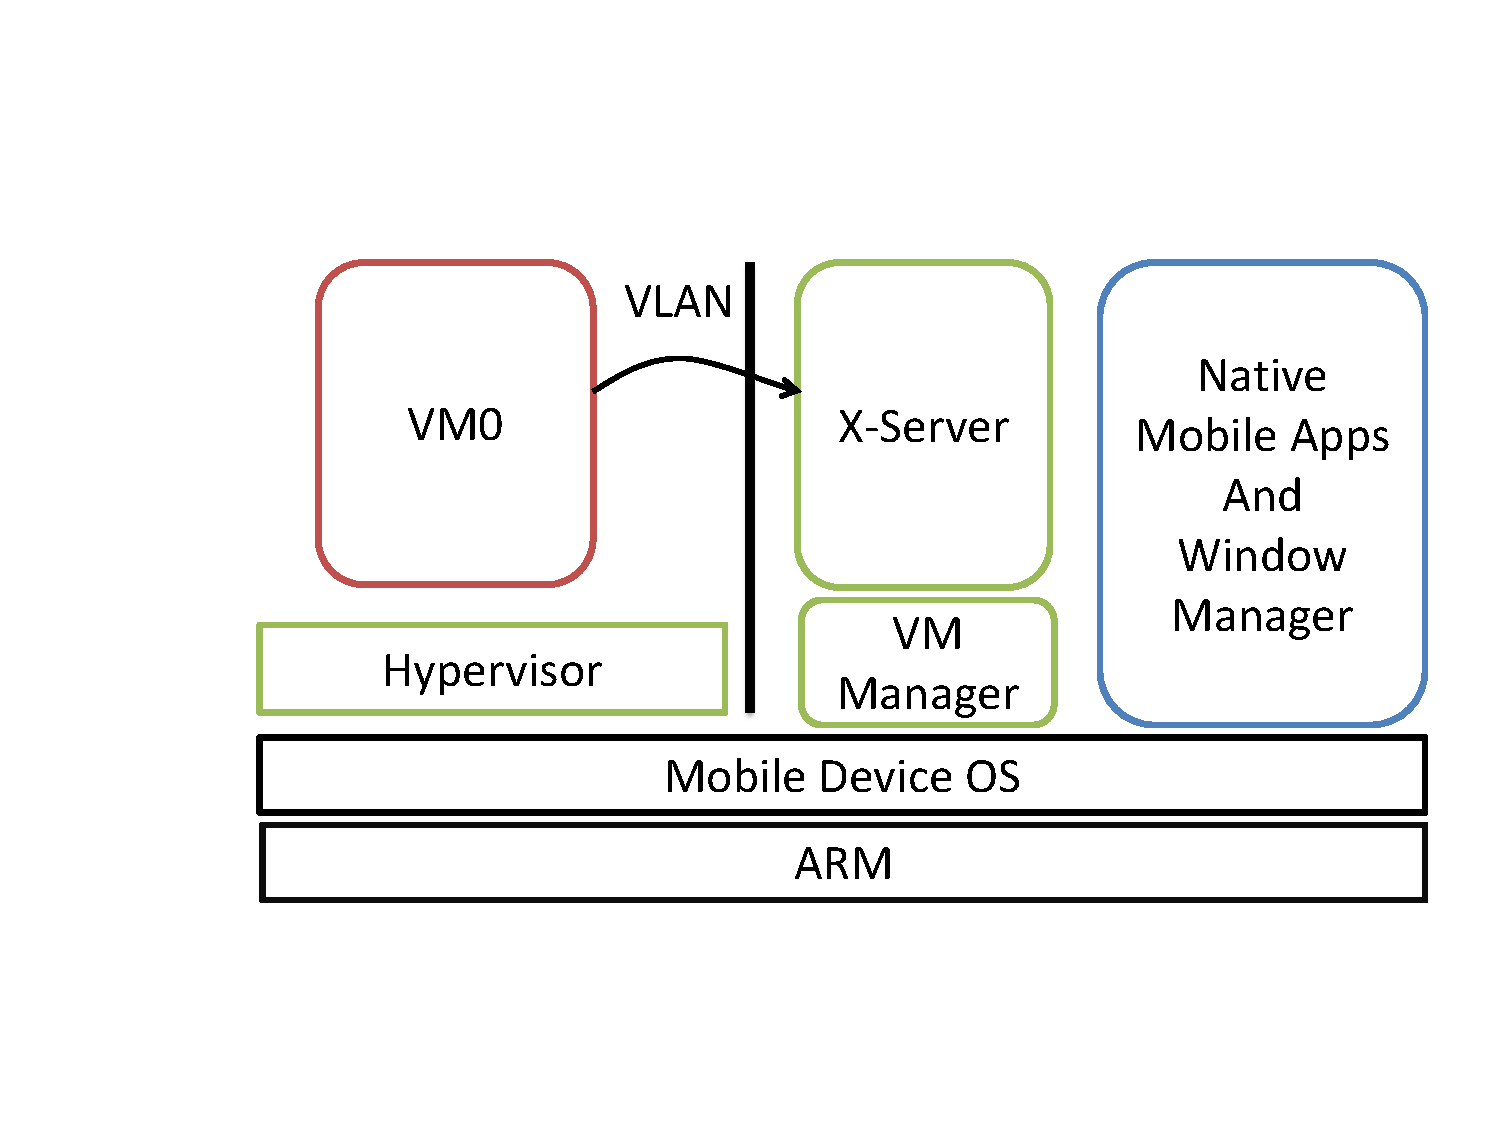
\includegraphics[width=1.0\columnwidth]{arch}
\caption{Architecture diagram}
\label{fig:arch}
\end{figure}

%% This subsection really needs a better title!
\subsection{Our solution}
We intend to improve upon the existing mobile virtualization solutions through superior usability.  By integrating with the host OS and building upon the existing user experience and bring added value to existing devices.
A primary goal of ours is compatibility with existing x86 and x11 applications such that upon our project completion we can immediately take advantage of the vast quantity of applications that already use these.
We also provide emulation which appears to the user to be at the application level, making it simpler conceptually to work with.
Our biggest contribution is the way we bring live migration into this.  This is the most novel part of our program.

{\bf NOTE: Add some discussion about power usage, memory constraints \newline}
